\section{Control System Design} \label{sec:part3}
In this section we want to design an autopilot for the ship. Which means we want to be able to choose an angle $\psi_r$ and the ship will follow this course. The model of the boat holds only for small deviations for the compass value. This means the compass value cannot be more than $\pm 35^{\circ}$. We used $\psi_r = 30$ in all the following simulations. We chose not to put a saturation on the output of the compass degree signal, this because we realized that the model always was within a boundary of $\pm$ 35 degrees.  

\subsection{PD controller}
In this subsection we start by designing a PD-controller in the form,
\begin{equation}
\begin{split}
   H_{pd}(s) = K_{pd} \frac{1+T_d s}{1+T_f s}
\end{split}
\label{eq:transferfunk}
\end{equation}
we base (\ref{eq:transferfunk}) on the transferfunction from $\delta$ to $\psi$ and assume that the disturbances are negligible. We let $\omega_c$ and the phase margin, $\varphi$, of the open loop system, $H_{pd}(s) \cdot H_{ship}(s)$, be approximately $0.10 \  (rad/s)$ and 50 degrees respectively. The systems transferfunction then becomes 
\begin{equation}
\begin{split}
    H_0(s) &= H_{pd}(s) \cdot H_{ship}(s) \\
    &= K_{pd} \frac{K + KT_d s}{s^3 T T_f +s^2(T + T_f) + s}
\end{split}
\end{equation}
\bigskip
We want $T_d$ to cancel out the transfer function time constant
\begin{align*}
    1 + T_d s &= 1 + Ts \\
    T_d &= T
\end{align*}
The transferfunction becomes, 
\begin{equation}
   H_{0}(s) = K_{pd} \frac{K}{(1+T_f s)s}
\end{equation}
To find the coefficient $T_f$ and $K_{pd}$, the cut-off frequency was given $\omega_c = 0.10 \ (rad/s)$, we solved the equation 
\begin{equation}
    \begin{split}
        1 &= |H_0(j\omega_{c})| \\
      \varphi &= 180 - \angle H_0(j\omega_c)
    \end{split}
\end{equation}
giving the expression for $T_f$ as
\begin{equation}
    T_f = \frac{1}{\omega_c\tan(\varphi*pi/180)}= 8.39099 
\end{equation}
The value for $K_{pd}$ is easily calculated from 
\begin{equation}
    K_{pd} = \frac{\sqrt{\omega_c^2 + T_f^2 \omega_c^4}}{K}= 0.836263
\end{equation}
The open loop system can be show in a bode diagram, see \cref{fig:bode}, with the phase margin approximately 50 degrees. $T_f$ affects the magnitude and phase of the system, while the $K_{pd}$ only affects the magnitude. This means that a lower $T_f$ make the response slower, while a bigger $T_f$ would make the response oscillate, maybe giving an overshoot. This is because $T_f$ limits the derivative effect.
\begin{figure}[H]
    \centering
    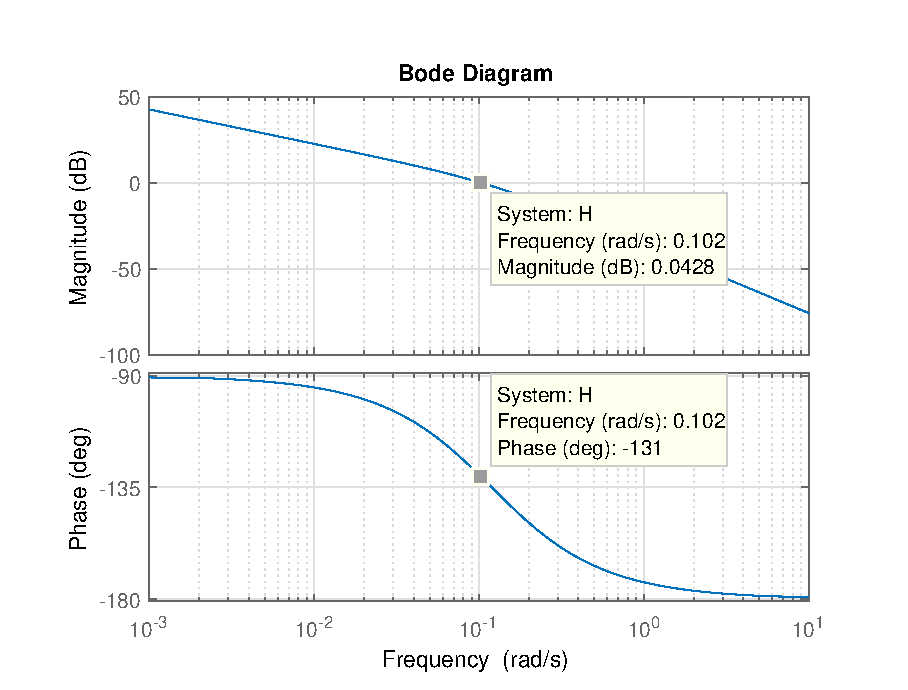
\includegraphics[width=0.75\linewidth]{Part3_pics/bode_nr2.eps}
    \caption{Bode diagram with $T_f$ = 8.391 and $K_{pd}$= 0.8363}
    \label{fig:bode}
\end{figure}



\subsection{Simulation with measurement noise}
Simulating the system without disturbances, except for measurement noise, we see that the autopilot manages to keep the reference, at $30^\circ$. For the Simulink- diagrams, see appendix \ref{sec:simulink_diagrams_3}

\begin{figure}[H]
    \centering
    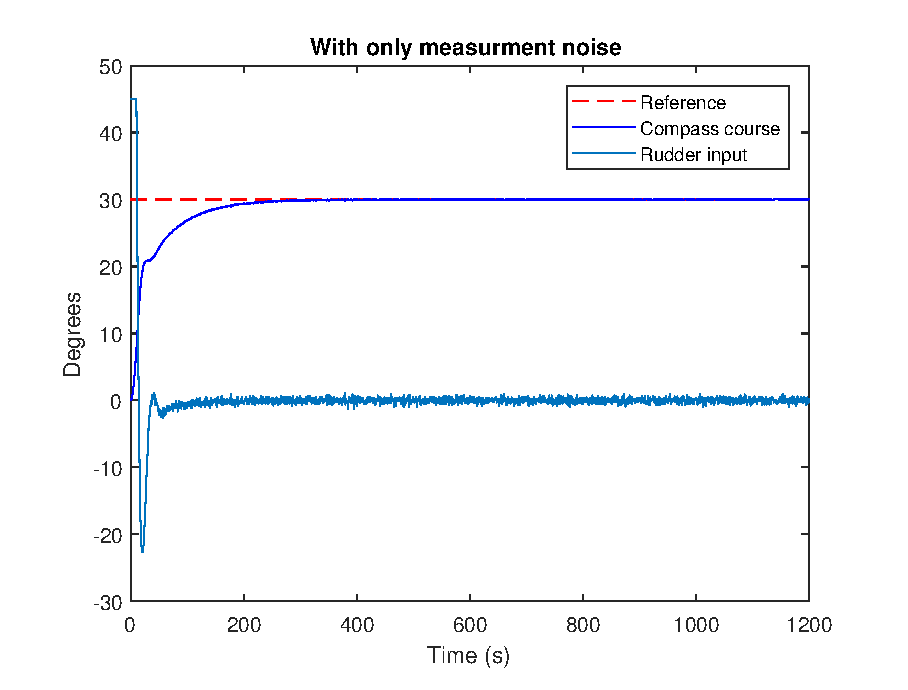
\includegraphics[width=0.6\linewidth]{Part3_pics/ny_3b.eps}
    \caption{Rudder and compass output of the system with measurment noise}
    \label{fig:p3b}
\end{figure}
In figure \ref{fig:p3b} we can observe that the compass course settles to 30 degrees pretty fast. The same goes for the rudder input, it holds 0 degrees. In the beginning of the plot we can observe that the rudder input goes in saturation. The autopilot work in the desired way in smooth weather conditions. This was also expected because the system is an ideal model and behave like the mathematical model. 

The ship use 300 seconds to achieve 30 degrees, if the system should be faster then the $K_{pd}$ must be increased. But if this is done the phase margin will decrease, this can make the system less stable. Notice that the rudder changes direction even though the system has reached its reference. This is because the course changes so fast and would end in an overshoot, so the derivative effect makes the system calm down by turning slower.



\subsection{Simulation with current disturbance} \label{p3c}
The system simulated with a current disturbance, but no wave disturbances is shown in \cref{fig:p3c} 
\begin{figure}[H]
    \centering
    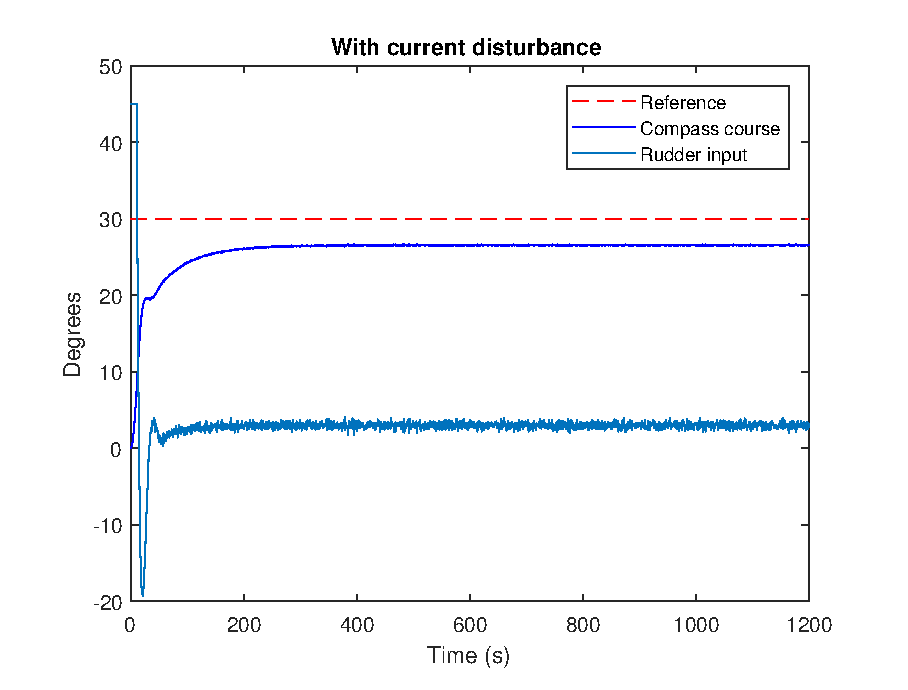
\includegraphics[width=0.6\linewidth]{Part3_pics/ny_3c.eps}
    \caption{Rudder and compass output of the system with measurement noise and current disturbance}
    \label{fig:p3c}
\end{figure}
In the figure \ref{fig:p3c}, there is a standard deviation equal 3.5 degrees from the reference on the compass course, and the rudder input is approximated 2.5 degrees. This is because the current is model as a constant disturbance. The error in the compass course is not desirable for an autopilot. The standard derivation in the compass is because the system has en PD regulator. For an better autopilot, we would make an PID to integrate up the error and reach the desired heading. 

\subsection{Simulation with wave disturbance}\label{p3d}
Simulating the system with a wave disturbance, but no current disturbances, we have a lot of noise, making it harder for the autopilot. The rudder tries to counter the effect each wave has on the ship. which means if will end up rapidly changing back and forth for each wave, unnecessarily compensating for the wave noise. 
\begin{figure}[H]
    \centering
    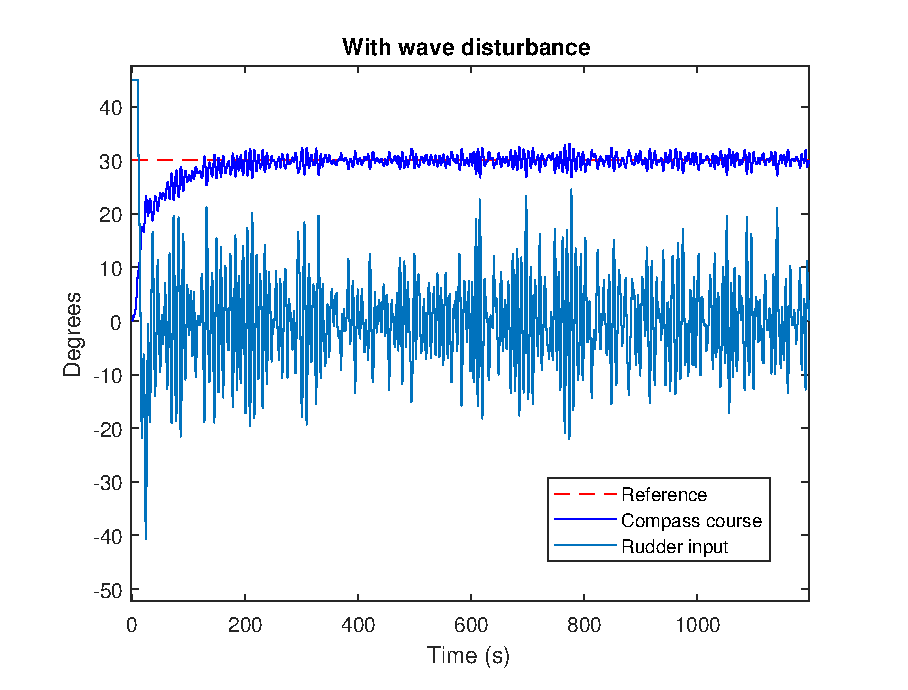
\includegraphics[width=0.6\linewidth]{Part3_pics/ny_3d.eps}
    \caption{Rudder and compass output of the system with measurement noise and wave disturbance}
    \label{fig:p3d}
\end{figure}
The wave disturbance is high frequency so it make the compass course oscillating round the reference point. In average the compass signal and rudder input, does not vary to much of the reference, so the ship would come to the desired destination. But the signals of the rudder input is not so precise in regards to the mechanical in the motor. To solve this we would recommend to make state estimators for the internal states. 